\section{Estimación de estado}
\label{sec:stateestimation}
La estimación de estado consiste en determinar el estado no medible de un sistema dinámico a partir de las mediciones de entrada y salida de dicho sistema, esto es, dado un estado inicial $\bm{x}_0$ y las observaciones $\bm{y}_1, \bm{y}_2, ..., \bm{y}_k$ conocidas en el tiempo $k$, el problema de estimación de estado en el paso de tiempo $k$ se basa en construir un estimador $\hat{\bm{x}}_k$ de $\bm{x}_k$.

Lamentablemente, las mediciones no son perfectas, lo que conduce a una inexactitud inherente en el valor de la medición. Para tener en cuenta estos errores, la estimación de estado procesa todas las mediciones disponibles y utiliza un \textit{análisis de regresión} para identificar el estado real probable del sistema.

\subsection{Filtro de Kalman}
El filtro de Kalman es un filtro Gaussiano con transición de estado y función de medición \textit{lineales}. Se le atribuye a {[\textbf{Kalman, 1960}]} y {[\textbf{Swerling, 1958}]} y se ha aplicado por primera vez al seguimiento por radar de objetivos aéreos, pero se ha utilizado en una gran cantidad de otros problemas de estimación desde entonces. El filtro de Kalman y sus diversos derivados son casi ubicuos en las aplicaciones de fusión de sensores.

El objetivo de este filtro, entonces, es computar $\{\hat{\bm{x}}_k,\hat{\bm{P}_k}\}$ utilizando toda la información disponible, incluyendo la presente en el tiempo $k$. Mientras el método de cuadrados mínimos recursivo actualiza la estimación de un parámetro estático, el filtro de Kalman es capaz de actualizar la estimación de un estado en evolución. Como se deriva del filtro general de Bayes{[\textbf{REF BAYES}]}, el objetivo de este filtro es tomar una estimación probabilística de este estado y actualizarla en tiempo real usando dos pasos, \textit{predicción} y \textit{corrección}.

Para poder entender mejor el filtro, se considera el problema de estimar la posición de un vehículo en una dimensión. Iniciando de una estimación probabilística en el tiempo $k-1$, el objetivo es predecir el nuevo estado mediante un modelo de moción, el cual puede ser derivado, por ejemplo, de la odometría de las ruedas o de las mediciones de una unidad inercial. Luego, con el modelo de observación derivado de, por ejemplo, los datos del GPS, se corrige esa predicción de la posición del vehículo en el tiempo $k$, tal como se observa en la Figura \ref{fig:kalmanfilter}. Cada una de estas componentes, la estimación inicial, el estado predicho, y el estado final corregido son todas variables aleatorias especificadas por sus valores medios y covarianzas. De este modo, puede pensarse al Filtro de Kalman como una técnica para fusionar información de diferentes sensores para producir una estimación final de un estado desconocido, tomando en cuenta incertidumbres en el moción y en las mediciones\footnote{Para identificar estados predichos de corregidos, por ejemplo en la matriz de covarianza $\bm{P}$, para el primer caso se utiliza la notación $\check{\bm{P}}$, mientras que para el segundo caso $\hat{\bm{P}}$.}.

\begin{figure}[!ht]
    \centering
    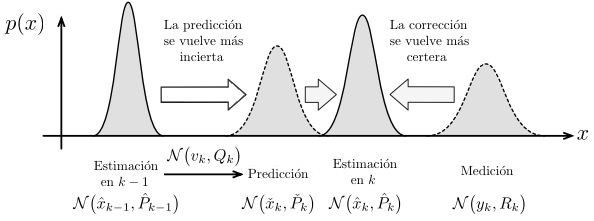
\includegraphics[width=\textwidth]{Img/KalmanFilter.png}
    \caption{Filtro de Kalman en una dimensión}
    \label{fig:kalmanfilter}
\end{figure}

En concreto, el filtro de Kalman requiere de un modelo de moción
\begin{equation}
    \bm{x}_k = \bm{F}_{k-1}\bm{x}_{k-1} + \bm{G}_{k-1}\bm{u}_{k-1} + \bm{w}_{k-1},
\end{equation}
y un modelo de medición lineal
\begin{equation}
    \bm{y}_k = \bm{H}_k\bm{x}_k + \bm{v}_k,
\end{equation}
siendo $\bm{u}_{k-1}$ una \textit{entrada de control} externa que afecta la evolución del estado del sistema, $\bm{v}_{k-1}$ el \textit{ruido de la medición} y $\bm{w}_{k-1}$ el \textit{rudo del proceso} que gobierna la incertidumbre de las entradas de control
\begin{equation}
    \bm{v}_k \sim \mathcal{N}(\bm{0},\bm{R}_k)\hspace{2cm}\bm{w}_k \sim \mathcal{N}(\bm{0},\bm{Q}_k)
\end{equation}

Puede decirse que el filtro de Kalman \textit{es muy similar a un estimador de cuadrados mínimos recursivo que incluye un modelo de moción} el cual indica cómo el estado evoluciona a través del tiempo. El mismo consta de dos pasos
\begin{enumerate}
    \item \textbf{Predicción}. Primero, se utiliza el modelo del proceso o moción para predecir como los estados evolucionaron desde el último paso de tiempo, y se propaga la incertidumbre.
    \begin{align}
        \check{\bm{x}}_k &= \bm{F}_{k-1}\bm{x}_{k-1}+\bm{G}_{k-1}\bm{u}_{k-1} \\
        \check{\bm{P}}_k &= \bm{F}_{k-1}\hat{\bm{P}}_{k-1}\bm{F}_{k-1}^T + \bm{Q}_{k-1}
    \end{align}
    \item \textbf{Actualización}. En el mismo se utiliza el modelo de medición y puede dividirse en dos pasos
    \begin{enumerate}
        \item \textit{Ganancia óptima}. Se utiliza la medición para corregir la predicción basada en el residuo o innovación de la medición y la ganancia óptima
        \begin{equation}
            \bm{K}_k = \check{\bm{P}}_{k}\bm{H}_k^T\left(\bm{H}_k\check{\bm{P}}_k\bm{H}_k^T + \bm{R}_k\right)^{-1}
        \end{equation}
        \item \textit{Corrección}. Se utiliza la ganancia para propagar la covarianza de estado de la predicción a la estimación corregida.
        \begin{align}
            \hat{\bm{x}}_k &= \check{\bm{x}}_k + \bm{K}_k\left(\bm{y}_k - \bm{H}_k\check{\bm{x}}_k\right) \\
            \hat{\bm{P}}_k &= (\bm{1} - \bm{K}_k\bm{H}_k)\check{\bm{P}}_k
        \end{align}
        siendo $(\bm{y}_k - \bm{H}_k\check{\bm{x}}_k)$ la llamada \textit{innovación de la medición}.
    \end{enumerate}
\end{enumerate}

Se dice que un estimador o filtro es \textit{insesgado} (en inglés, \textit{unbiased}) si produce un error promedio de cero para todo paso de tiempo k
\begin{equation}
    E[\hat{p}_k-p_k] = 0
\end{equation}
donde $\hat{p}_k$ denota al valor estimado y $p_k$ al valor verdadero.

Considerando la dinámica de error, siendo el error de estado predicho
\begin{equation}
    \check{\bm{e}}_k = \check{\bm{x}}_k - \bm{x}_k
\end{equation}
y el error de estimación corregido
\begin{equation}
    \hat{\bm{e}}_k = \hat{\bm{x}}_k - \bm{x}_k
\end{equation}
se puede obtener mediante el uso de las ecuaciones del filtro de Kalman que
\begin{align}
    \check{\bm{e}}_k &= \bm{F}_{k-1}\check{e}_{k-1} - \bm{w}_k \\
    \check{\bm{e}}_k &= \left(\bm{1} - \bm{K}_k\bm{H}_k\right)\check{\bm{e}}_k + \bm{K}_k\bm{v}_k
\end{align}

Si se tiene ruido blanco no correlacionado con media cero y
\begin{equation*}
    E[\hat{\bm{e}}_0] = \bm{0}\hspace{0.5cm}\land\hspace{0.5cm}E[\bm{v}] = \bm{0}\hspace{0.5cm}\land\hspace{0.5cm}E[\bm{w}] = \bm{0}
\end{equation*}
se llega a que el valor esperado de estos errores es cero para todo $k$
\begin{align}
    E[\check{\bm{e}}_k] &= \bm{F}_{k-1}E[\check{\bm{e}}_{k-1}] - E[\bm{w}_k] = \bm{0} \\
    E[\hat{\bm{e}}_k] &= \left(\bm{1} - \bm{K}_k\bm{H}_k\right)E[\check{\bm{e}}_k] + \bm{K}_k E[\bm{v}_k] = \bm{0}
\end{align}

Por consistencia se dice a que, para todos los pasos de tiempo $k$, la covarianza del filtro, $P_k$, equivale al valor esperado del cuadrado del error
\begin{equation}
    E[\hat{e}_k^2] = E[(\hat{p}_k - p_k)^2] = \hat{P}_k
\end{equation}
Esto quiere decir que el filtro no es ni demasiado seguro (optimista) ni inseguro respecto a la estimación que ha producido.

Se puede demostrar que, si se tiene ruido blanco y
\begin{equation*}
    E[\hat{\bm{e}}_0\hat{\bm{e}}_0^T] = \check{\bm{P}}_0\hspace{0.5cm}\land\hspace{0.5cm}E[\bm{v}] = \bm{0}\hspace{0.5cm}\land\hspace{0.5cm}E[\bm{w}] = \bm{0}
\end{equation*}
las predicciones serán consistentes
\begin{equation*}
    E[\check{\bm{e}}_k\check{\bm{e}}_k^T] = \check{\bm{P}_k}\hspace{1cm}\land\hspace{1cm}E[\hat{\bm{e}}_k\hat{\bm{e}}_k^T] = \hat{\bm{P}}_k
\end{equation*}

En conclusión, si el ruido es blanco no correlacionado con media cero, el filtro de Kalman es \textit{no sesgado} y \textit{consistente}. Debido a estos dos hechos, se dice que el filtro de Kalman es el \textit{mejor estimador lineal no sesgado} (o \textit{BLUE} por sus siglas en inglés), ya que produce estimaciones no sesgadas con la menor varianza posible.

\subsection{Filtro de Kalman extendido}
Si bien el filtro de Kalman es el mejor estimador lineal no sesgado, por lo general los sistemas reales no son lineales. El concepto principal del filtro de Kalman extendido es el de linealizar un sistema no lineal, esto es, elegir un punto de operación $a$ y hallar una aproximación lineal a la función no lineal en la vecindad del punto. En dos dimensiones refiere a encontrar la recta tangente, por ejemplo. Se llega a esto matemáticamente realizando la serie de Taylor de la función y tomando solo los términos de primer orden, esto es
\begin{equation}
    f(x)\approx f(a) + \frac{\delta f(x)}{\delta x}\bigg\rvert_{x=a}(x-a)
\end{equation}

Para el caso del filtro de Kalman extendido, se elige como punto de operación al estimador de estado más reciente, entonces, el modelo de moción linealizado
\begin{equation}
    \begin{aligned}
        \bm{x}_k &= \bm{f}_{k-1}(\bm{x}_{k-1},\bm{u}_{k-1},\bm{w}_{k-1})\\
        &\approx \bm{f}_{k-1}(\hat{\bm{x}}_{k-1},\bm{u}_{k-1},\bm{0}) + \bm{F}_{k-1}\left(\bm{x}_{k-1} - \hat{\bm{x}}_{k-1}\right) + \bm{L}_{k-1}\bm{w}_{k-1}
    \end{aligned}
    \label{eq:linearizedmotionmodel}
\end{equation}
y el modelo de medición linealizado
\begin{equation}
    \bm{y}_k = \bm{h}_k(\bm{x}_k,\bm{v}_k)\approx \bm{h}_k(\check{\bm{x}}_k,\bm{0}) + \bm{H}_k(\bm{x}_k - \check{\bm{x}}_k) + \bm{M}_k \bm{v}_k
    \label{eq:linearizedmeasurementmodel}
\end{equation}
siendo
\begin{align}
    \bm{F}_{k-1} &= \frac{\delta \bm{f}_{k-1}}{\delta \bm{x}_{k-1}}\bigg\rvert_{\hat{\bm{x}}_{k-1},\bm{u}_{k-1},\bm{0}} \\
    \bm{L}_{k-1} &= \frac{\delta \bm{f}_{k-1}}{\delta \bm{w}_{k-1}}\bigg\rvert_{\hat{\bm{x}}_{k-1},\bm{u}_{k-1},\bm{0}} \\
    \bm{H}_k &= \frac{\delta \bm{h}_k}{\delta \bm{x}_k}\bigg\rvert_{\check{\bm{x}}_{k},\bm{0}} \\
    \bm{M}_k &= \frac{\delta \bm{h}_k}{\delta \bm{v}_k}\bigg\rvert_{\check{\bm{x}}_{k}\bm{0}}
\end{align}
las llamadas matrices Jacobianas del sistema.

Finalmente, teniendo en cuenta los modelos linealizados y las matrices Jacobianas, se llega a los pasos del filtro de Kalman extendido
\begin{enumerate}
    \item \textbf{Predicción}
        \begin{align}
            \check{\bm{x}}_k &= \bm{f}_{k-1}(\hat{\bm{x}}_{k-1},\bm{u}_{k-1},\bm{0})\\
            \check{\bm{P}}_k &= \bm{F}_{k-1}\hat{\bm{P}}_{k-1}\bm{F}_{k-1}^T + \bm{L}_{k-1}\bm{Q}_{k-1}\bm{L}_{k-1}^T
        \end{align}
    \item \textbf{Actualización}
    \begin{enumerate}
        \item \textit{Ganancia óptima}
            \begin{equation}
                \bm{K}_k = \check{\bm{P}}_k\bm{H}_k^T(\bm{H}_k\check{\bm{P}}_k\bm{H}_k^T + \bm{M}_k\bm{R}_k\bm{M}_k^T)^{-1}
            \end{equation}
        \item \textit{Correción}
            \begin{align}
                \hat{\bm{x}}_k &= \check{\bm{x}}_k + \bm{K}_k(\bm{y}_k - \bm{h}_k(\check{\bm{x}}_k,\bm{0}))\\
                \hat{\bm{P}}_k &= (\bm{1} - \bm{K}_k\bm{H}_k)\check{\bm{P}}_k
            \end{align}
    \end{enumerate}
\end{enumerate}

\subsection{Filtro de Kalman extendido de error de estado}
Supóngase que se tiene el estado verdadero $\bm{x}$, el cual se quiere estimar, mientras que el estado nominal $\hat{\bm{x}}$ es la mejor estimación de lo que podría ser el estado verdadero basado en lo que se conoce del modelo de moción y las entradas de control. Como el modelo de moción no es perfecto, y el hecho de que exista ruido aleatorio del proceso, estos errores se acumulan con el tiempo a medida que se integra el modelo de moción. A partir de esto, puede plantearse un \textit{error de estado} $\delta \bm{x}$ como el lugar donde todos estos errores de modelado y ruidos del proceso se acumulan con el tiempo, por lo que el error de estado es la diferencia entre el estado nominal y el estado verdadero
\begin{equation}
    \bm{x} = \hat{\bm{x}} + \delta \bm{x}
\end{equation}
tal como se observa en la Figura \ref{fig:errorstate}.

\begin{figure}[!h]
    \centering
    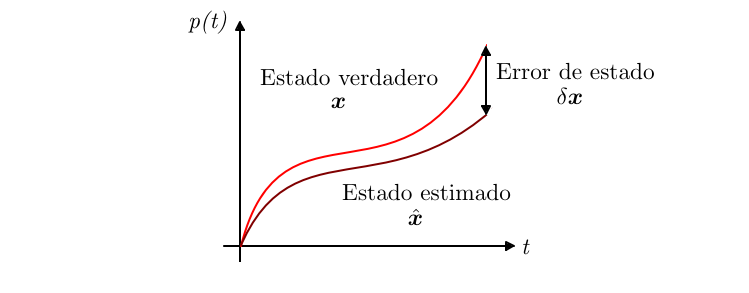
\includegraphics[width=\textwidth]{Img/ErrorState.png}
    \caption{El error de estado como la diferencia entre el estado verdadero y el estado estimado}
    \label{fig:errorstate}
\end{figure}

Puede decirse que el ''largo'' estado nominal realiza un seguimiento de lo que el modelo de movimiento predice que debería ser el estado, mientras que el ''pequeño'' error de estado captura los errores de modelado y el ruido del proceso que se acumula con el tiempo. Si se puede estimar el error de estado, lo cual se consigue mediante una \textit{linealización local}\footnote{El filtro de Kalman extendido convencional, en cambio, estima el estado completo}, el mismo puede utilizarse para corregir al estado nominal, consiguiendo así una mejor estimación.

En lugar de realizar el filtro de Kalman en el estado completo, el cual puede tener muchos comportamientos no lineales complicados, se busca con este filtro estimar el error de estado, para luego utilizar el estimador de este error de estado como una corrección al estado nominal. El error de estado es más dócil al filtrado lineal que el de estado nominal, el que puede integrarse de forma no lineal. Además de esto, permite trabajar con cantidades restringidas (por ejemplo, rotaciones en tres dimensiones).

Las Expresiones (\ref{eq:linearizedmotionmodel}) y (\ref{eq:linearizedmeasurementmodel}) pueden reescribirse, entonces, como
\begin{align}
    \delta \bm{x}_k &= \bm{F}_{k-1}\delta\bm{x}_{k-1} + \bm{L}_{k-1}\bm{w}_{k-1} \\
    \bm{y}_k &= \bm{h}_k(\check{\bm{x}}_k,\bm{0}) + \bm{H}_k\delta\bm{x}_k + \bm{M}_k\bm{v}_k 
\end{align}
donde
\begin{align}
    \delta \bm{x}_k &= \bm{x}_k - \bm{f}_{k-1}(\hat{\bm{x}}_{k-1},\bm{u}_{k-1},\bm{0}) = \bm{x}_k - \check{\bm{x}}_k \\
    \delta\bm{x}_{k-1} &= \bm{x}_{k-1} - \hat{\bm{x}}_{k-1}
\end{align}

Es posible utilizar esta formulación del error de estado de una forma muy similar al filtro de Kalman extendido visto anteriormente
\begin{enumerate}
    \item \textit{Actualizar el estado nominal con el modelo de moción}
    \begin{equation}
        \check{\bm{x}}_k = \bm{f}_{k-1}(\bm{x}_{k-1},\bm{u}_{k-1},\bm{0})
    \end{equation}
    donde $\bm{x}_{k-1}$ se trata del mejor estimador actual, pudiendo ser tanto $\hat{\bm{x}}$ como $\check{\bm{x}}$.
    \item \textit{Propagar incertidumbres}
    \begin{equation}
        \check{\bm{P}}_k = \bm{F}_{k-1}\bm{P}_{k-1}\bm{F}_{k-1}^T + \bm{L}_{k-1}\bm{Q}_{k-1}\bm{L}_{k-1}^T
    \end{equation}
    donde $\bm{P}_{k-1}$ se trata del mejor estimador actual.
    \item \textit{Si no se tiene una medición disponible, volver al paso anterior, caso contrario}
    \begin{enumerate}
        \item Computar la ganancia de Kalman
        \begin{equation}
            \bm{K}_k = \check{\bm{P}}_k\bm{H}_k^T(\bm{H}_k\check{\bm{P}}_k\bm{H}_k^T + \bm{R})^{-1}
        \end{equation}{}
        \item Computar el mejor estimador del error de estado
        \begin{equation}
            \delta\hat{\bm{x}}_k = \bm{K}_k(\bm{y}_k - \bm{h}_k(\check{\bm{x}}_k,\bm{0}))
        \end{equation}
        \item Corregir el estado nominal
        \begin{equation}
            \hat{\bm{x}}_k = \check{\bm{x}}_k + \delta\hat{\bm{x}}_k
        \end{equation}
        \item Actualizar la covarianza de estado
        \begin{equation}
            \hat{\bm{P}}_k = (\bm{1} - \bm{K}_k\bm{H}_k)\check{\bm{P}}_k
        \end{equation}
    \end{enumerate}
\end{enumerate}

El filtro de Kalman extendido en las dos variantes desarrolladas linealiza los modelos de moción y medición no lineal para actualizar la media y covarianza del estado. La diferencia entre la aproximación lineal y la función no lineal se denomina \textit{error de linealización}. En general, este error depende de 
\begin{itemize}
    \item qué tan no lineal es la función. Si la misma varía poco a medida que pasa el tiempo, la aproximación será buena. En cambio, si varía rápidamente, la aproximación presentará errores considerables respecto a la verdadera.
    \item qué tan lejos se está del punto de operación elegido. Mientras más lejos se esté de dicho punto, más probable es que la aproximación lineal diverja de la función verdadera.
\end{itemize}

Esto puede llevar a que tanto la media estimada del estado como la covarianza estimada del mismo no puedan obtener precisamente la incertidumbre verdadera en el estado, haciendo que \textit{el estimador tenga un exceso de confianza en una respuesta incorrecta}. En el peor de los casos, esto puede producir que el estimador diverja, haciendo que el filtro tenga que reinicializarlo en caso de ser posible, ya que no puede corregirse.

\subsection{Transformada ''unscented'' o de punto sigma}
La transformación ''unscented''  \textbf{Julier y Uhlmann (4)} \textbf{Wan y van derMerwe (8)} es un método utilizado para calcular los primeros momentos de la densidad de distribución de probabilidad de una variable aleatoria. ''Resulta más fácil aproximar una distribución Gaussiana que aproximar una transformación no lineal arbitraria.'' \textbf{J. K. Uhlmann (7)}. Esta transformada consta de tres pasos
\begin{enumerate}
    \item Un conjunto de puntos, conocidos como \textit{puntos sigma}, se eligen de la distribución de entrada de forma tal que sean un cierto número de divisiones estándar separados de la media. En general, para una función densidad de probabilidad de $N$ dimensiones, se necesitan $2N + 1$ puntos sigma, uno para la media y el resto distribuidos simétricamente sobre la media. Para la ubicación de cada uno, hay que seguir una serie de pasos
    \begin{enumerate}
        \item Calcular la descomposición de Cholesky de la matriz de covarianza asociada con la distribución de entrada. Esta descomposición es prácticamente una operación de raíz cuadrada.
        \begin{equation}
            \bm{L}\bm{L}^T = \bm{\Sigma}_{xx}
        \end{equation}
        \item Una vez que se descompuso la matriz de covarianza, puede elegirse el primer punto sigma para que sea la media de la distribución y el resto a que sea la media más o menos algún factor multiplicado por cada componente de la matriz $\bm{L}$ obtenida en la descomposición de Cholesky
        \begin{align}
            \bm{x}_0 &= \bm{\mu}_0 \\
            \bm{x}_i &= \bm{\mu}_i + \sqrt{N+\kappa}\ col_i\bm{L} \\
            \bm{x}_{i+N} &= \bm{\mu}_x - \sqrt{N+\kappa}\ col_i\bm{L}
        \end{align}
        con $i = 1, ..., N$ y $\kappa$ es un parámetro de ajuste que, por ejemplo, para distribuciones Gaussianas, asignar $\kappa = 3 - N$ es una buena elección.
    \end{enumerate}
    \item Una vez elegidos los puntos sigma, siendo
    \begin{equation}
        \bm{y}_i = \bm{h}(\bm{x}_i)
    \end{equation}
    con $i = 1, ..., 2N$, se aplica la función no lineal a cada uno de estos puntos elegidos, produciendo un nuevo set de puntos transformados, pertenecientes a la distribución resultante.
    
    \item Finalmente, se computa la media muestral y la covarianza de los puntos sigma resultantes con pesos elegidos cuidadosamente, y esto dará una buena aproximación de la media y covarianza de la distribución de salida verdadera.
    \begin{align}
        \bm{\mu}_y &= \sum_{i=0}^{2N}\alpha_i\bm{y}_i \\
        \bm{\Sigma}_{yy} &= \sum_{i=0}^{2N}\alpha_i(\bm{y}_i-\bm{\mu}_y)(\bm{y}_i-\bm{\mu}_y)^T
    \end{align}
\end{enumerate}
siendo $\alpha_i$ los pesos asociados para cada uno de los puntos
\begin{align}
    \alpha_i = \frac{\kappa}{N+\kappa}\hspace{1cm}\text{para}\hspace{1cm}i &= 0 \\
    \alpha_i = \frac{0.5}{N+\kappa}\hspace{1cm}\text{para}\hspace{1cm}i &\neq 0
\end{align}

\subsection{Filtro de Kalman ''unscented''}
A diferencia del filtro de Kalman extendido ordinario y el de error de estado, en el filtro de Kalman ''unscented'', o también conocido como el \textit{filtro de Kalman de punto sigma}, en lugar de linealizar las ecuaciones del sistema, se utiliza la transformada ''unscented'' para aproximar la función densidad de probabilidad directamente. Las etapas del filtro, como es de esperarse, difieren en parte del resto:
\begin{enumerate}
    \item \textbf{Etapa de predicción}. Para propagar el estado desde el tiempo $k-1$ al tiempo $k$, se aplica la transformada ''unscented'' utilizando el mejor estimador actual de la media y la covarianza
    \begin{enumerate}
        \item \textit{Obtener los puntos sigma}
        \begin{align}
            \hat{\bm{L}}_{k-1}\hat{\bm{L}}_{k-1}^T &= \hat{\bm{P}}_{k-1}^T \\
            \hat{\bm{x}}_{k-1}^{(0)} &= \hat{\bm{x}}_{k-1} \\
            \hat{\bm{x}}_{k-1}^{(i)} &= \hat{\bm{x}}_{k-1} + \sqrt{N+\kappa}\ col_i\hat{\bm{L}}_{k-1} \\
            \hat{\bm{x}}_{k-1}^{(i+N)} &= \hat{\bm{x}}_{k-1} - \sqrt{N+\kappa}\ col_i\hat{\bm{L}}_{k-1}            
        \end{align}
        con $i=1,...,N$.
        \item \textit{Propagar los puntos sigma}
        \begin{equation}
            \check{\bm{x}}_k^{(i)} = \bm{f}_{k-1}\left(\hat{\bm{x}}_{k-1}^{(i)},\bm{u}_{k-1},\bm{0}\right)
        \end{equation}
        con $i=0,...,2N$.
        \item \textit{Computar la media y covarianza predicha}
        \begin{align}
            \alpha^{(i)} &= \frac{\kappa}{N+\kappa}\hspace{1cm}\text{para}\hspace{1cm}i = 0 \\
            \alpha^{(i)} &= \frac{0.5}{N+\kappa}\hspace{1cm}\text{para}\hspace{1cm}i \neq 0 \\
            \check{\bm{x}}_k &= \sum_{i=0}^{2N}\alpha^{(i)}\check{\bm{x}}_k^{(i)} \\
            \check{\bm{P}}_k &= \sum_{i=0}^{2N}\alpha^{(i)}\left(\check{\bm{x}}_k^{(i)} - \check{\bm{x}}_k\right)\left(\check{\bm{x}}_k^{(i)} - \check{\bm{x}}_k\right)^T + \bm{Q}_{k-1}
        \end{align}
        siendo $\bm{Q}_{k-1}$ el ruido del proceso aditivo\footnote{En caso de no ser aditivo, la ecuación cambia.}.
    \end{enumerate}
    \item \textbf{Etapa de corrección}. Para corregir el estimador de estado utilizando las mediciones en el tiempo $k$, se utiliza el modelo de medición no lineal y los puntos sigma de la etapa de predicción para predecir las mediciones
    \begin{enumerate}
        \item \textit{Predecir mediciones de los puntos sigma redibujados}\footnote{Redibujados, ya que se agregó el ruido del proceso al final del último paso, lo que modificará las posiciones de algunos de los puntos sigma.}.
        \begin{equation}
            \hat{\bm{y}}_k^{(i)} = \bm{h}_k\left(\check{\bm{x}}_k^{(i)},\bm{0}\right)
        \end{equation}
        con $i = 0, ..., 2N$.
        \item \textit{Estimar la media y covarianza de las mediciones predichas}
        \begin{align}
            \hat{\bm{y}}_k &= \sum_{i=0}^{2N}\alpha^{(i)}\hat{\bm{y}}_k^{(i)} \\
            \bm{P}_y &= \sum_{i=0}^{2N}\alpha^{(i)}\left(\hat{\bm{y}}_k^{(i)} - \hat{\bm{y}}_k\right)\left(\hat{\bm{y}}_k^{(i)} - \hat{\bm{y}}_k\right)^T + \bm{R}_k
        \end{align}
        siendo $\bm{R}_k$ ruido de la medición aditivo\footnote{Al igual que en la etapa anterior, esto solo es válido para ruido aditivo}.
        \item \textit{Computar la covarianza cruzada y la ganancia de Kalman}
        \begin{align}
            \bm{P}_{xy} &= \sum_{i=0}^{2N}\alpha^{(i)}\left(\check{\bm{x}}_k^{(i)} -  \check{\bm{x}}_k\right)\left(\hat{\bm{y}}_k^{(i)} -  \hat{\bm{y}}_k\right)^T \\
            \bm{K}_k &= \bm{P}_{xy}\bm{P}_y^{-1}
        \end{align}
        \item \textit{Calcular la media y varianza corregidas}
        \begin{align}
            \hat{\bm{x}}_k &= \check{\bm{x}}_k + \bm{K}_k\left(\bm{y}_k - \hat{\bm{y}}_k\right) \\
            \hat{\bm{P}}_k &= \check{\bm{P}}_k - \bm{K}_k\bm{P}_y\bm{K}_k^T
        \end{align}
    \end{enumerate}
\end{enumerate}

Si bien este filtro presentado suele presentar un mejor rendimiento, el costo computacional es levemente superior al resto de los desarrollados debido a la transformada que realiza.

\subsection{Filtro de Kalman en ROS}
Como el filtro de Kalman (en cualquiera de sus versiones) es de gran utilidad a la hora de la fusión sensorial, el mismo, entre otras aplicaciones, suele ser utilizado en ROS para determinar la pose del robot en base a los datos de sus sensores. Dentro de los paquetes que pueden realizar esto, caben destacar a
\begin{itemize}
    \item \textit{robot\_pose\_ekf}\footnote{\url{http://wiki.ros.org/robot_pose_ekf}}, el cual utiliza un Filtro de Kalman extendido para realizar el cálculo de la pose. Presenta como desventaja que sólo puede tener dos datos de odometría y uno de una unidad inercial, aunque suele ser suficiente en gran parte de las aplicaciones.
    \item \textit{robot\_localization}\footnote{\url{http://wiki.ros.org/robot_localization}}, el cual da la opción de calcular la pose mediante un Filtro de Kalman extendido o un Filtro de Kalman unscented. El mismo, a diferencia del robot\_pose\_ekf, permite cualquier número de odometrías y datos de unidades sensoriales distintas, además de contar con una mayor flexibilidad y personalización que el mencionado anteriormente.
\end{itemize}


% \begin{huge}
% SACARLO AL FDP!
% \end{huge}
% \subsection{Filtro de partículas}
% \textbf{[QUE SE YO, MIRAR TULSYAN, 2016 Y VER QUE HACER O QUE NO, YA ME SUPERO]}

% A diferencia del filtro de Kalman, el filtro de partículas representa la distribución de probabilidad \textbf{(O CDF???? MIRAR [TULSYAN, 2016])}\footnote{Las PDF pueden tener valores mayores a 1, mientras que las CDF no} como un set de muestras (partículas)
% \begin{equation}
%     p(x) \simeq \frac{1}{N} \sum_i \delta_{x^{(i)}}(dx)
% \end{equation}
% donde $\delta_{x^{(i)}}(dx)$ es la función impulso centrada en $x^{(i)}$ evaluando un intervalo infinitesimal de longitud $dx$, como puede observarse en la Figura \ref{fig:probabilityinfinitesimal}. Mientras más densas sean las muestras $x^{(i)}$ en una región, mayor será la probabilidad de que el estado actual caiga dentro de esa región. Este método puede representar cualquier distribución arbitraria, ya que busca una buena aproximación de dicha distribución, en lugar de representarla de un modo simplificado, como es el caso de filtro de Kalman (Gaussiana).
% \begin{figure}
%     \centering
%     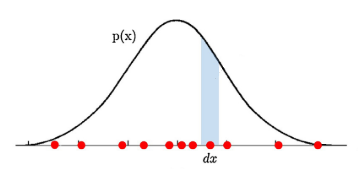
\includegraphics{Img/ProbabilityInfinitesimal.png}
%     \caption{Densidad de probabilidad seccionada}
%     \label{fig:probabilityinfinitesimal}
% \end{figure}{}

% A continuación se presenta el denominado \textit{algoritmo de muestreo de importancia secuencial} (SIS) para el filtro de partículas, que incluye un paso de remuestreo en cada instante. 

% El filtro de partículas, entonces, es un método de Monte Carlo secuencial\textbf{[REF O LO PONGO?]} que busca representar la probabilidad posterior $p(x_k|y_{1:k})$ por un set de partículas $x_k^i$ cada una con sus pesos asociados $w_k^i$, con $i=1,...,N_s$, siendo $N_s$ el número de partículas. Para lograr esto, se utiliza el denominado \textit{algoritmo de muestreo de importancia secuencial} (SIS) para el filtro de partículas
% \begin{equation}
%     p(x_k|y_{1:k}) \approx \sum_{i=1}^{N_s}w_k^{(i)}\delta_{x_k^{(i)}}(dx_k)
% \end{equation}
% siendo $w_k^{(i)}$ los \textit{pesos de importancia} asociados a $x_k^{(i)}$, estando los mismos normalizados para que $\sum_i w_k^i = 1$. Como no se tiene una representación explícita de la probabilidad posterior, el algoritmo SIS utiliza una \textit{densidad de importancia} para hallar las muestras, que es una densidad propuesta para representar otra que no puede calcularse exactamente. Luego, las muestras se extraen de la densidad de importancia en lugar de la densidad real. Para dicho propósito, suele utilizarse el prior $p(x)$, y luego de cada muestra muestreada se actualiza el \textit{peso de importancia}
% \begin{equation}
%     w = 
% \end{equation}
% basado en las observaciones realizadas.

% Un problema común con el filtro de partículas SIS es el fenómeno de la degeneración, donde después de unos pocos estados, todas las partículas menos una tendrán un peso insignificante [1,4,8-18]. Esta degeneración implica que se dedica un gran esfuerzo computacional a actualizar las partículas cuya contribución a la aproximación de la función de densidad posterior es casi cero. Este problema se puede superar aumentando el número de partículas, o más eficientemente seleccionando adecuadamente la densidad de importancia como la densidad anterior. Además, se recomienda el uso de la técnica de remuestreo para evitar la degeneración de las partículas.

% \subsection{Filtro de Partículas en ROS}
% Los filtros de partículas (en sus distintas versiones) suelen utilizarse para aplicaciones de mapeo 2D, en el que involucran un LIDAR 2D y, en ciertos casos, sensores adicionales. Como ejemplos de esto pueden destacarse los paquetes \textit{amcl}\footnote{\url{http://wiki.ros.org/amcl}} y \textit{hector\_slam}\footnote{\url{http://wiki.ros.org/hector_slam}}.